\chapter{The Gate: Crowd or Record?}
\label{sec:gate}
\lhead{\emph{Chapter 6. The Gate}}  % page header

This chapter asks whether acceptance at ICLR favours papers that follow the crowd or papers anchored to their authors'
own earlier work.

\section{Is following the crowd associated with acceptance?}
Table~\ref{tab:gate} and Figure~\ref{fig:gate} collect the tests at the gate. Of those in the figure, crowding was
registered, title style had been explored before registration and the remaining tests were found post hoc in
discovery; each held-out test was declared before any held-out estimate for its question was computed.

The registered crowding test predicted a penalty for crowded topics, and it is uninformative. Per log unit of crowding
(the natural log of one plus the number of the topic's earlier papers), acceptance changes by $-$1.68\,pp [$-$3.68,
+0.32] in discovery and by $-$1.51 [$-$5.20, +2.19] on held-out papers, against an MDE80 of 4.8. In short, the data show no clear penalty or premium, although held-out premiums above +2.19\,pp per log unit lie outside the interval.

The clearest sign of imitation in the corpus is in title style. The share of titles that open with a short coined
name and a colon rose from 10.9\% in 2017 to 44.6\% in 2026. Within topic and year, with contribution-type, FM and
team-size controls, such branded titles are accepted 1.74\,pp [+0.37, +3.11] more often in discovery, but this estimate
is not a test, since title style had been explored before registration. The declared held-out test gives +1.76
[$-$0.82, +4.34] (one-sided $p = 0.089$); the held-out test is uninformative (below its MDE80 of 3.2), so the premium
remains \lab{exploratory}. Raw within-year gaps are larger (+3.3 in discovery and +4.0 on held-out papers); about half
of each gap is explained by topic, contribution type, FM use and team size. Titles can also be revised after the
decision, which could create such a premium.

FM papers are accepted 4.62\,pp more often [+2.79, +6.44], with no sign of a difference between late and early adopters: the premium changes by +0.19 [$-$0.96, +1.34] per logit unit of the topic's prior FM adoption (that is,
per unit of its log-odds). Both results are \lab{exploratory}, and they fit efficient choice as well as imitation, if
review rewards it. A topic's \emph{edge} is its acceptance rate minus that of all other papers of the same year, using
topics of the 2017--2020 map. The edge persists but shrinks towards the mean: among discovery papers, the 2018--2022
edge predicts the 2024--2026 edge with slope 0.38 [0.18, 0.58]. The held-out test asks a related but different
question, namely whether the discovery edges for 2018--2022 predict the 2024--2026 edges of held-out papers; it gives a
slope of 0.60 [0.32, 0.88] and is \lab{held-out supported}. A favoured topic thus keeps only part of its edge, as
expected when decisions carry a large arbitrary component \citep{cortes2021inconsistency,beygelzimer2023has}.

Keyword timing shows at most weak associations, and we treat it as \lab{exploratory}: keyword popularity had been
explored against acceptance before registration, and both held-out intervals below include zero. On held-out papers,
\emph{Emerging} keywords (young and rising) are associated with higher acceptance than \emph{Mainstream} keywords (old
and flat), by +3.25 [$-$0.18, +6.69], and acceptance may fall after a keyword's share peaks ($-$5.2 [$-$11.1, +0.7];
$-$1.7 without the six keywords examined before this test was declared). Neither pattern shows the constant premium for
popular keywords that imitation would predict if review rewarded it.

\begin{table}[tb]
\centering
\footnotesize
\setlength{\tabcolsep}{3pt}
\renewcommand{\arraystretch}{1.1}
\begin{tabularx}{\textwidth}{@{}Y L{2.7cm} L{2.7cm} L{2.4cm}@{}}
\toprule
Contrast in acceptance & Discovery [95\% CI] & Held-out [95\% CI] & Label \\
\midrule
\multicolumn{4}{@{}l}{\textit{Referenced to the team's own record}} \\
Far jump: 10th percentile of \Fmax{} $-$ median & $-$5.44\newline[$-$7.10, $-$3.78] & $-$6.09\newline[$-$9.32,
$-$2.86] & \lab{held-out supported} \\
Same author, 0.1 closer in cosine similarity$^c$ & +0.55\newline[+0.21, +0.90] & +1.06\newline[+0.23, +1.89] &
\lab{held-out supported} \\
One topic insider vs none$^c$ & +3.42\newline[+1.18, +5.66] & +3.88\newline[+0.28, +7.47] & \lab{held-out supported} \\
\addlinespace
\multicolumn{4}{@{}l}{\textit{Referenced to others or the field}} \\
Crowding, per log unit$^a$ & $-$1.68\newline[$-$3.68, +0.32] & $-$1.51\newline[$-$5.20, +2.19] & \lab{uninformative} \\
Branded title$^b$ & +1.74\newline[+0.37, +3.11] & +1.76\newline[$-$0.82, +4.34] & \lab{exploratory} \\
Change in FM premium per logit unit of prior adoption & +0.19\newline[$-$0.96, +1.34] & -- & \lab{exploratory} \\
Topic edge 2018--22 \ra{} 2024--26, slope$^c$ & 0.38\newline[0.18, 0.58] & 0.60\newline[0.32, 0.88] & \lab{held-out
supported} \\
Emerging $-$ Mainstream keyword$^{b,c}$ & +2.67\newline[+0.76, +4.58] & +3.25\newline[$-$0.18, +6.69] &
\lab{exploratory} \\
Distance from earlier ICLR work: least-distant fifth $-$ middle fifth & $-$3.27\newline[$-$4.93, $-$1.60] &
$-$0.13\newline[$-$3.50, +3.25] & \lab{uninformative} \\
\bottomrule
\end{tabularx}
\caption[Acceptance contrasts at the gate]{Acceptance contrasts at the gate, in pp within topic and year (topic edges
and keywords: against the same year's other papers). Rows differ in population and unit, so their sizes are not
comparable. Held-out tests are one-sided. $^a$Registered; predicted a penalty; MDE80 4.8. $^b$Explored against
acceptance before registration. For titles the discovery estimate is not a test (held-out MDE80 3.2); for keywords it
is a declared post hoc test on a dimension already seen. $^c$Holm-adjusted $p$ across the six secondary held-out tests:
topic-edge slope 0.019, edge prediction 0.026, same-author closeness 0.026, insider 0.052, Emerging keywords 0.063,
same-author distance slope 0.22.}
\label{tab:gate}
\end{table}

\begin{figure}[tb]
  \centering
  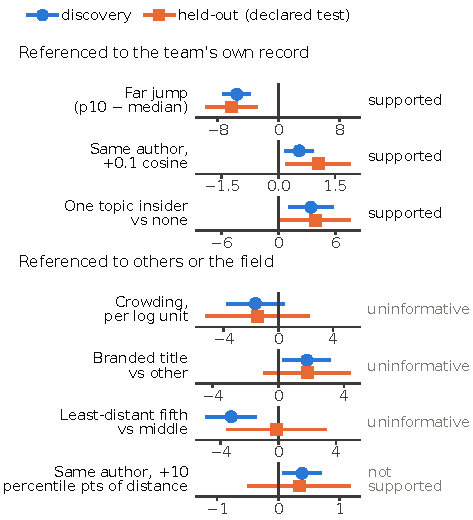
\includegraphics[width=0.72\textwidth]{figs/fig4_gate.pdf}
  \caption[Gate tests by reference point]{Gate tests by reference point: discovery estimates (blue circles) and
  declared held-out tests (orange squares), with 95\% intervals. The held-out verdict is shown at right: `supported' means
  \lab{held-out supported}; `uninformative' means not supported and below the test's MDE80; `not supported' marks a
  declared test without a registered MDE80, which we call inconclusive. Each row has its own scale: pp for the far
  jump (closeness at its 10th percentile, p10, minus the median), the insider, the branded title and the least-distant
  fifth; pp per log unit for crowding; and pp per 0.1 cosine similarity and per 10 percentile points of distance for
  the two same-author slopes. Because the scales differ, compare verdicts rather than sizes.}
  \label{fig:gate}
\end{figure}

\section{What is acceptance associated with?}
The main pattern is the \emph{far jump}: the lower acceptance of papers far from the team's earlier work. Among
20,430 decided 2023--2026 papers with an experienced author, acceptance at the 10th percentile of closeness to the
team's own record is 5.44\,pp lower than at the median in discovery ($-$5.44 [$-$7.10, $-$3.78]) and 6.09\,pp lower on
held-out papers ($-$6.09 [$-$9.32, $-$2.86]), with power = 0.89. This was the primary test declared for the held-out
papers, and it is \lab{held-out supported}. Adjusted acceptance rises with closeness up to the fourth quintile. The far
jump remains with a newcomer control ($-$5.0), although closeness is correlated with newcomer status ($r = -0.57$).

Holding the author fixed, a paper 0.1 closer in cosine similarity to that author's earlier work is associated with
acceptance 0.55\,pp higher [+0.21, +0.90] in discovery and 1.06\,pp higher [+0.23, +1.89] on held-out papers. This
result is \lab{held-out supported} and survives a family-wise correction across the secondary tests. Controls for
newcomer status and for co-authors' experience change it little (+0.48 and +0.50), though unmeasured differences in
co-author quality could also bias it; a simulation run before the held-out test showed that such a confounder can
shift the estimate. In a related within-author comparison, on a paper in a topic new to them, the same author's
acceptance is 1.37\,pp lower ($-$1.37 [$-$2.74, $-$0.004]; author fixed effects, \lab{exploratory}).\footnote{Newcomer
papers as a whole have 10.2\,pp lower acceptance ($-$10.2 [$-$11.8, $-$8.7]) within topic and year
(\lab{exploratory}), but that gap mostly reflects who writes them: it shrinks once team size and the authors' ICLR
experience are controlled, and shrinks further within the same authors.}

Having one topic insider on the team, rather than none, is associated with acceptance 3.42\,pp higher [+1.18, +5.66] in
discovery and 3.88\,pp higher [+0.28, +7.47] on held-out papers, at fixed team size and number of experienced authors
(\lab{held-out supported}). The result does not survive the family-wise correction (Holm-adjusted $p = 0.052$), and
status explains it equally well: each additional insider adds only 0.58\,pp more than each additional experienced
author from another topic ($p = 0.16$; \lab{exploratory}).

Distance from earlier ICLR work as a whole gives uninformative results. In the same SPECTER2 embedding space, papers in
the least-distant fifth differ from those in the middle fifth by $-$3.27 [$-$4.93, $-$1.60] in discovery but by $-$0.13
[$-$3.50, +3.25] on held-out papers, a test with power = 0.47. The within-author slope for distance from earlier ICLR
work was not supported either, and with no MDE80 available it is inconclusive. Of the distance-based tests, only the
associations with the team's own earlier work held up on held-out papers.

\section{Interpretation}
These associations all involve closeness to the team's own earlier work, as continuity predicts, but expertise,
evaluator conservatism and visible status predict them as well \citep{li2017expertise,merton1968matthew}. Double-blind
review does not rule status out: where reviewers can see the authors, famous authors fare better
\citep{tomkins2017reviewer}, and preprints can reveal who wrote a paper \citep{bharadhwaj2020deanonymization}.

% ===============================================================================================================
